%!TeX root = ../My_thesis.tex


% .---|||___|||--- C H A P T E R ---|||___|||---. %
\chapter{Аппробация разработанной модели и её модификаций}
% .---|||___|||--- C H A P T E R ---|||___|||---. %


% .---|||___|||--- S E C T I O N ---|||___|||---. %
\section{Метрики для оценки модели упрощения}
% .---|||___|||--- S E C T I O N ---|||___|||---. %


Для перевода текстов (в том числе и упрощения) довольно часто используют метрку BLEU.
В оригинальной статье Папинени и др.~\cite{BLEU} показали наличие корреляции данной метрики с сохранением грамматики и смысла переведённых предложений.

Однако есть и более специфичная метрика, разработанная специально для автоматического упрощения текстов "--- SARI~\cite{SARI}.
Она, по сравнению BLEU, лучше коррелирует с упрощением предложений, а также с сохранением лексической и структурной частей предложений.

Вообще говоря, метрика BLEU не очень хорошо подходит для задачи упрощения текстов~\cite{bleu-is-dogshit}.
Однако во всех источниках, посвящённых упрощению текстов, рассмотренных в данной работе, приводились обе метрики (BLEU~и~SARI), поэтому и мы поступим аналогично, но будем отдавать метрике SARI больший приоритет.


% .---|||___|||--- S E C T I O N ---|||___|||---. %
\section{Результаты}
% .---|||___|||--- S E C T I O N ---|||___|||---. %


Результаты метрик BLUE и SARI для изначальной модели и вариантов её улучшения представлены в~\taref{metrics}.

\begin{table}[H]% Пример оформления таблицы
  \centering\small
  \caption{Метрики полученных моделей}
  \label{metrics}
    \begin{tabular}{|l|l|l|}
      \hline
      \textbf{Модель} & \textbf{BLEU} & \textbf{SARI} \\ \hline
      Transformer & 46{,}98 & 64{,}57 \\ \hline
      Pretrained Transformer & 51{,}12 & 67{,}89 \\ \hline
      Pretrained Encoder & 48{,}22 & 65{,}67 \\ \hline
    \end{tabular}
    \normalsize
\end{table}

В~\taref{metrics} введены следующие обозначения:
\begin{itemize}%
  \item Transformer "--- изначальная модель;
  \item Pretrained Transformer "--- предобученная модель, которую дообучаем, замедляя обучение encoder'а;
  \item Pretrained Encoder "--- изначальная модель, в которой заменяем encoder на предобученный, замедляя его обучение.
\end{itemize}

По~\taref{metrics} видно, что наиболее успешной оказалсь модель Pretrained Transformer "--- улучшение по сравнению с изначальной моделью на 4{,}14\% и 3{,}32\% для BLEU и SARI соответственно.
Это может говорить о том, что предобучение положительно сказывается и на decoder'е, так как упрощение в основном оставляет предложение в исходном виде, за исключением упрощённых его частей.


% .---|||___|||--- S E C T I O N ---|||___|||---. %
\section{Гистограммы и доверительные интервалы}
% .---|||___|||--- S E C T I O N ---|||___|||---. %


Рассмотрим гистограммы распределения значений метрик BLUE и SARI для изначальной модели (Transformer) и улучшенной версии (Pretrained Transformer) "--- см.~\firef{metrics-comparison}.
Можно увидеть, как в левой части гистограмм (худшие показатели метрик) доминирует первая модель, на правой же части (лучшие показатели метрик) "--- модифицированная.

\begin{figure}[H]%
  \centering%
  \caption{Сравнение гистограмм метрик BLEU~(a) и SARI~(b) \\ жёлтый "--- Transformer, синий "--- Pretrained Transformer}
  \label{metrics-comparison}
  \begin{subfigure}[H]{0.45\textwidth}
    \label{bleu-part}
    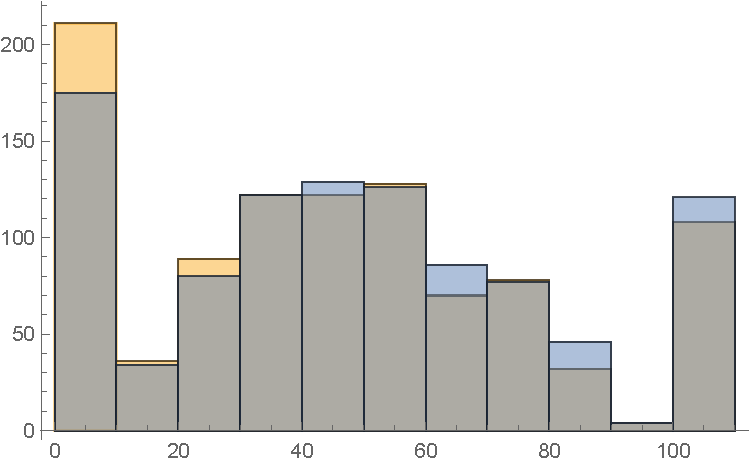
\includegraphics[width=\textwidth]{bleu-comparison.pdf}
    \caption{Метрики BLEU}
  \end{subfigure}
  \begin{subfigure}[H]{0.45\textwidth}
    \label{sari-part}
    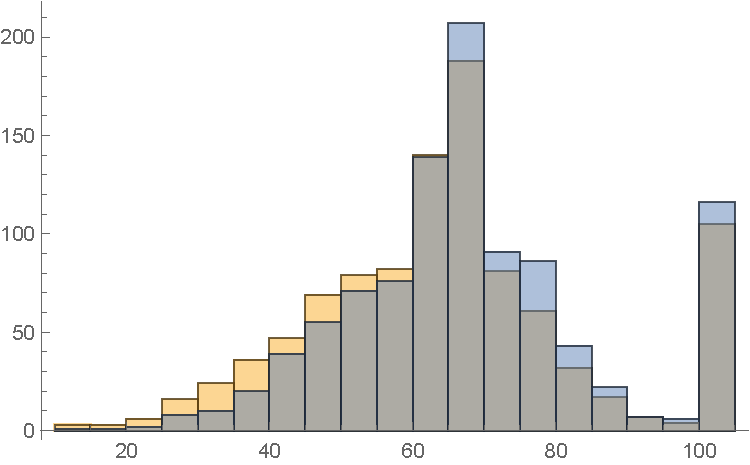
\includegraphics[width=\textwidth]{sari-comparison.pdf}
    \caption{Метрики SARI}
  \end{subfigure}
\end{figure}%

Это может говорить о том, что улучшение модели действительно положительно влияет на полученные показания метрик, однако для большей уверенности в этой гипотезе вычислим доверительные интервалы для этих значений и посмотрим, не пересекаются ли они.
Так как мы имеем большой размер выборки (1\,000~элементов), примем гипотезу о нормальном распределении этой выборки и будем считать доверительные интервалы по следующей формуле:
\begin{equation}%
  \label{ci-formula}
  CI = \mu \pm p \frac{\sigma}{\sqrt{N}},
\end{equation}
где
\begin{itemize}%
  \item $CI$ "--- доверительные интервалы,
  \item $\mu$ "--- среднее значение выборки,
  \item $p$ "--- вероятность попадания истинного значения в доверительные интервалы (в данной работе возьмём значение $0{,}95$),
  \item $\sigma$ "--- среднеквадратическое отклонение выборки,
  \item $N$ "--- количество элементов в выборке (в данной работе "--- 1\,000).
\end{itemize}

Вычислим доверительные интервалы\footnote{Заметим, что среднее значение для метрик BLEU отличается от указанных значений в~\taref{metrics}. Связано это с тем, что метрика BLEU вычисляется иным образом для набора предложений, в отличие от единичных предложений, однако разность между значениями при единичных вычислениях ниже, в то время как доверительные интервалы не пересекаются, что говорит о том, что и доверительные интервалы для значений со всеми предложениями не пересекаются. В случае же с SARI разницы никакой нет.}:
\begin{equation}\label{bleu-ci}%
  CI_{\text{Transformer (BLEU)}} = 43{,}85 \pm 0{,}95, \
  CI_{\text{Pretrained Transformer (BLEU)}} = 47{,}37 \pm 0{,}94,
\end{equation}
\begin{equation}\label{sari-ci}%
  CI_{\text{Transformer (SARI)}} = 64{,}57 \pm 0{,}55, \
  CI_{\text{Pretrained Transformer (SARI)}} = 67{,}89 \pm 0{,}51.
\end{equation}

В итоге получаем расстояние между нижней границей Pretrained Transformer и верхней границей Transformer в $1{,}63$ и $2{,}26$ для метрик BLEU и SARI соответственно, что может говорить о явном различии истинных значений метрик BLUE и SARI для изначальной и модифицированной моделей.
А это, в свою очередь, говорит о наличии значимости внесённых изменений в модель со статистической точки зрения.


% .---|||___|||--- S E C T I O N ---|||___|||---. %
\section{Примеры упрощения предложений изначальной и модифицированной моделями}
% .---|||___|||--- S E C T I O N ---|||___|||---. %


Рассмотрим примеры предложений из корпуса для тестирования, упрощение которых улучшилось благодаря модификции модели.

В примере на~\firef{simplificationComparison} упрощается слово \jp{内気} на более простое \jp{気が弱い}.
Однако изначальная модель немного не справилась с упрощением "--- \jp{弱い}~(слабая) вместо \jp{気が弱い}~(скромная)\footnote{Здесь также происходит упрощение слова \jp{ますます} (на \jp{さらに} "--- более распространённое слово), однако обе модели упростили его одинаково, поэтому не будем заострять на этом внимание.}.

\begin{figure}[H]%
  \centering
  \begin{tabular}{l}
    (1) исходное предложение \\  
    \yubi{\jp{彼女}}{kanojo}
    \yubi{\jp{は}}{wa}
    \yubi{\jp{内気}}{uchiki}
    \yubi{\jp{な}}{na}
    \yubi{\jp{ので}}{node}
    \yubi{\jp{、}}{}
    \yubi{\jp{ますます}}{masumasu}
    \yubi{\jp{彼女}}{kanojo}
    \yubi{\jp{が}}{ga}
    \yubi{\jp{好き}}{suki}
    \yubi{\jp{だ}}{da} \\ 
    пер. "--- она робкая, из-за чего я люблю её ещё больше \\ 
    (2) изначальная модель \\ 
    \yubi{\jp{彼女}}{kanojo}
    \yubi{\jp{は}}{wa}
    \yubi{\jp{弱い}}{\textbf{yowai}}
    \yubi{\jp{ので}}{node}
    \yubi{\jp{、}}{}
    \yubi{\jp{さら}}{sara}
    \yubi{\jp{に}}{ni}
    \yubi{\jp{彼女}}{kanojo}
    \yubi{\jp{が}}{ga}
    \yubi{\jp{好き}}{suki}
    \yubi{\jp{だ}}{da} \\ 
    пер. "--- она \textbf{слабая}, из-за чего я люблю её ещё больше \\ 
    (3) модифицированная модель (Pretrained Transformer) \\  
    \yubi{\jp{彼女}}{kanojo}
    \yubi{\jp{は}}{wa}
    \yubi{\jp{気}}{\textbf{ki}}
    \yubi{\jp{が}}{\textbf{ga}}
    \yubi{\jp{弱い}}{\textbf{yowai}}
    \yubi{\jp{ので}}{node}
    \yubi{\jp{、}}{}
    \yubi{\jp{さら}}{sara}
    \yubi{\jp{に}}{ni}
    \yubi{\jp{彼女}}{kanojo}
    \yubi{\jp{が}}{ga}
    \yubi{\jp{好き}}{suki}
    \yubi{\jp{だ}}{da} \\
    пер. "--- она \textbf{скромная}, из-за чего я люблю её ещё больше \\ 
  \end{tabular}
  \caption{Пример улучшения упрощения предложения \\ \jp{彼女は内気なので、ますます彼女が好きだ}}
  \label{simplificationComparison}
\end{figure}

Рассмотрим ещё один пример "--- см.~\firef{simplificationComparison2}.
Здесь есть непереводимый на русский язык нюанс упрощения "--- \jp{我}~(литературное «я»)~$\to$~\jp{自分}~(обычное «я»)\footnote{Это именно тот самый случай многообразия японских местоимений (о котором мы говорили в первой главе), каждое из которых несёт свой оттенок и имеет своё место в использовании в японском языке, в русском же языке есть лишь одно слово "--- «я».}.
Заметим также, что в изначальной модели искажается исходный смысл предложения (хотя предложение и упрощается), в модифицированной же модели этот смысл сохраняется (упрощение также производится).

\begin{figure}[H]%
  \centering
  \begin{tabular}{l}
    (1) исходное предложение \\  
    \yubi{\jp{彼}}{kare}
    \yubi{\jp{は}}{wa}
    \yubi{\jp{怒り}}{okori}
    \yubi{\jp{に}}{ni}
    \yubi{\jp{我}}{ware}
    \yubi{\jp{を}}{wo}
    \yubi{\jp{忘れた}}{wasureta} \\ 
    пер. "--- он забылся в гневе \\ 
    (2) изначальная модель \\ 
    \yubi{\jp{彼}}{kare}
    \yubi{\jp{は}}{wa}
    \yubi{\jp{怒っている}}{okotteiru}
    \yubi{\jp{のに}}{noni}
    \yubi{\jp{自分}}{\textbf{jibun}}
    \yubi{\jp{の}}{no}
    \yubi{\jp{意見}}{\textbf{iken}}
    \yubi{\jp{を}}{\textbf{wo}}
    \yubi{\jp{忘れた}}{\textbf{wasureta}} \\ 
    пер. "--- он хоть и разозлился, но \textbf{забыл своё мнение} \\ 
    (3) модифицированная модель (Pretrained Transformer) \\  
    \yubi{\jp{彼}}{kare}
    \yubi{\jp{は}}{wa}
    \yubi{\jp{怒っている}}{okotteiru}
    \yubi{\jp{こと}}{koto}
    \yubi{\jp{に}}{ni}
    \yubi{\jp{自分}}{\textbf{jibun}}
    \yubi{\jp{を}}{wo}
    \yubi{\jp{忘れた}}{wasureta} \\ 
    пер. "--- он забылся, из-за того что разозлился \\ 
  \end{tabular}
  \caption{Пример улучшения упрощения предложения \\ \jp{彼は怒りに我を忘れた}}
  \label{simplificationComparison2}
\end{figure}

Рассмотрим ещё один пример упрощения "--- \firef{simplificationComparison3}.
Здесь можно увидеть упомянутое в первой главе упрощение сложного слова (\jp{入場料}), состоящего из кандзи, перефразированием более простыми словами (возможно, не самым красивым и лаконичным образом, но значительно более простым).
Однако изначальная модель, опять, же исказила смысл предложения, в то время как модель модифицированная передала изначальный посыл.

\begin{figure}[H]%
  \centering
  \begin{tabular}{l}
    (1) исходное предложение \\  
    \yubi{\jp{入}}{nyuu}
    \yubi{\jp{場}}{jou}
    \yubi{\jp{料}}{ryou}
    \yubi{\jp{は}}{wa}
    \yubi{\jp{ただ}}{tada}
    \yubi{\jp{だった}}{datta} \\ 
    пер. "--- вход был бесплатным \\ 
    (2) изначальная модель \\ 
    \yubi{\jp{入る}}{hairu}
    \yubi{\jp{ため}}{tame}
    \yubi{\jp{の}}{no}
    \yubi{\jp{お金}}{okane}
    \yubi{\jp{は}}{wa}
    \yubi{\jp{ただ}}{tada}
    \yubi{\jp{なかった}}{nakatta} \\ 
    пер. "--- деньги для входа не были бесплатными \\ 
    (3) модифицированная модель (Pretrained Transformer) \\  
    \yubi{\jp{入る}}{hairu}
    \yubi{\jp{ため}}{tame}
    \yubi{\jp{の}}{no}
    \yubi{\jp{お金}}{okane}
    \yubi{\jp{は}}{wa}
    \yubi{\jp{0}}{zero}
    \yubi{\jp{円}}{en}
    \yubi{\jp{だった}}{datta} \\ 
    пер. "--- денег для входа нужно было 0 йен \\ 
  \end{tabular}
  \caption{Пример улучшения упрощения предложения \\ \jp{入場料はただだった}}
  \label{simplificationComparison3}
\end{figure}


% % .---|||___|||--- S E C T I O N ---|||___|||---. %
% \section{Примеры упрощения разработанной системой}
% % .---|||___|||--- S E C T I O N ---|||___|||---. %


% Посмотрим на несколько примеров упрощения разработанной системой, а также улучшенной версии.


